% Options for packages loaded elsewhere
\PassOptionsToPackage{unicode}{hyperref}
\PassOptionsToPackage{hyphens}{url}
%
\documentclass[
]{book}
\usepackage{lmodern}
\usepackage{amsmath}
\usepackage{ifxetex,ifluatex}
\ifnum 0\ifxetex 1\fi\ifluatex 1\fi=0 % if pdftex
  \usepackage[T1]{fontenc}
  \usepackage[utf8]{inputenc}
  \usepackage{textcomp} % provide euro and other symbols
  \usepackage{amssymb}
\else % if luatex or xetex
  \usepackage{unicode-math}
  \defaultfontfeatures{Scale=MatchLowercase}
  \defaultfontfeatures[\rmfamily]{Ligatures=TeX,Scale=1}
\fi
% Use upquote if available, for straight quotes in verbatim environments
\IfFileExists{upquote.sty}{\usepackage{upquote}}{}
\IfFileExists{microtype.sty}{% use microtype if available
  \usepackage[]{microtype}
  \UseMicrotypeSet[protrusion]{basicmath} % disable protrusion for tt fonts
}{}
\makeatletter
\@ifundefined{KOMAClassName}{% if non-KOMA class
  \IfFileExists{parskip.sty}{%
    \usepackage{parskip}
  }{% else
    \setlength{\parindent}{0pt}
    \setlength{\parskip}{6pt plus 2pt minus 1pt}}
}{% if KOMA class
  \KOMAoptions{parskip=half}}
\makeatother
\usepackage{xcolor}
\IfFileExists{xurl.sty}{\usepackage{xurl}}{} % add URL line breaks if available
\IfFileExists{bookmark.sty}{\usepackage{bookmark}}{\usepackage{hyperref}}
\hypersetup{
  pdftitle={A Minimal Book Example},
  pdfauthor={Yihui Xie},
  hidelinks,
  pdfcreator={LaTeX via pandoc}}
\urlstyle{same} % disable monospaced font for URLs
\usepackage{color}
\usepackage{fancyvrb}
\newcommand{\VerbBar}{|}
\newcommand{\VERB}{\Verb[commandchars=\\\{\}]}
\DefineVerbatimEnvironment{Highlighting}{Verbatim}{commandchars=\\\{\}}
% Add ',fontsize=\small' for more characters per line
\usepackage{framed}
\definecolor{shadecolor}{RGB}{248,248,248}
\newenvironment{Shaded}{\begin{snugshade}}{\end{snugshade}}
\newcommand{\AlertTok}[1]{\textcolor[rgb]{0.94,0.16,0.16}{#1}}
\newcommand{\AnnotationTok}[1]{\textcolor[rgb]{0.56,0.35,0.01}{\textbf{\textit{#1}}}}
\newcommand{\AttributeTok}[1]{\textcolor[rgb]{0.77,0.63,0.00}{#1}}
\newcommand{\BaseNTok}[1]{\textcolor[rgb]{0.00,0.00,0.81}{#1}}
\newcommand{\BuiltInTok}[1]{#1}
\newcommand{\CharTok}[1]{\textcolor[rgb]{0.31,0.60,0.02}{#1}}
\newcommand{\CommentTok}[1]{\textcolor[rgb]{0.56,0.35,0.01}{\textit{#1}}}
\newcommand{\CommentVarTok}[1]{\textcolor[rgb]{0.56,0.35,0.01}{\textbf{\textit{#1}}}}
\newcommand{\ConstantTok}[1]{\textcolor[rgb]{0.00,0.00,0.00}{#1}}
\newcommand{\ControlFlowTok}[1]{\textcolor[rgb]{0.13,0.29,0.53}{\textbf{#1}}}
\newcommand{\DataTypeTok}[1]{\textcolor[rgb]{0.13,0.29,0.53}{#1}}
\newcommand{\DecValTok}[1]{\textcolor[rgb]{0.00,0.00,0.81}{#1}}
\newcommand{\DocumentationTok}[1]{\textcolor[rgb]{0.56,0.35,0.01}{\textbf{\textit{#1}}}}
\newcommand{\ErrorTok}[1]{\textcolor[rgb]{0.64,0.00,0.00}{\textbf{#1}}}
\newcommand{\ExtensionTok}[1]{#1}
\newcommand{\FloatTok}[1]{\textcolor[rgb]{0.00,0.00,0.81}{#1}}
\newcommand{\FunctionTok}[1]{\textcolor[rgb]{0.00,0.00,0.00}{#1}}
\newcommand{\ImportTok}[1]{#1}
\newcommand{\InformationTok}[1]{\textcolor[rgb]{0.56,0.35,0.01}{\textbf{\textit{#1}}}}
\newcommand{\KeywordTok}[1]{\textcolor[rgb]{0.13,0.29,0.53}{\textbf{#1}}}
\newcommand{\NormalTok}[1]{#1}
\newcommand{\OperatorTok}[1]{\textcolor[rgb]{0.81,0.36,0.00}{\textbf{#1}}}
\newcommand{\OtherTok}[1]{\textcolor[rgb]{0.56,0.35,0.01}{#1}}
\newcommand{\PreprocessorTok}[1]{\textcolor[rgb]{0.56,0.35,0.01}{\textit{#1}}}
\newcommand{\RegionMarkerTok}[1]{#1}
\newcommand{\SpecialCharTok}[1]{\textcolor[rgb]{0.00,0.00,0.00}{#1}}
\newcommand{\SpecialStringTok}[1]{\textcolor[rgb]{0.31,0.60,0.02}{#1}}
\newcommand{\StringTok}[1]{\textcolor[rgb]{0.31,0.60,0.02}{#1}}
\newcommand{\VariableTok}[1]{\textcolor[rgb]{0.00,0.00,0.00}{#1}}
\newcommand{\VerbatimStringTok}[1]{\textcolor[rgb]{0.31,0.60,0.02}{#1}}
\newcommand{\WarningTok}[1]{\textcolor[rgb]{0.56,0.35,0.01}{\textbf{\textit{#1}}}}
\usepackage{longtable,booktabs}
\usepackage{calc} % for calculating minipage widths
% Correct order of tables after \paragraph or \subparagraph
\usepackage{etoolbox}
\makeatletter
\patchcmd\longtable{\par}{\if@noskipsec\mbox{}\fi\par}{}{}
\makeatother
% Allow footnotes in longtable head/foot
\IfFileExists{footnotehyper.sty}{\usepackage{footnotehyper}}{\usepackage{footnote}}
\makesavenoteenv{longtable}
\usepackage{graphicx}
\makeatletter
\def\maxwidth{\ifdim\Gin@nat@width>\linewidth\linewidth\else\Gin@nat@width\fi}
\def\maxheight{\ifdim\Gin@nat@height>\textheight\textheight\else\Gin@nat@height\fi}
\makeatother
% Scale images if necessary, so that they will not overflow the page
% margins by default, and it is still possible to overwrite the defaults
% using explicit options in \includegraphics[width, height, ...]{}
\setkeys{Gin}{width=\maxwidth,height=\maxheight,keepaspectratio}
% Set default figure placement to htbp
\makeatletter
\def\fps@figure{htbp}
\makeatother
\setlength{\emergencystretch}{3em} % prevent overfull lines
\providecommand{\tightlist}{%
  \setlength{\itemsep}{0pt}\setlength{\parskip}{0pt}}
\setcounter{secnumdepth}{5}
\usepackage{booktabs}
\ifluatex
  \usepackage{selnolig}  % disable illegal ligatures
\fi
\usepackage[]{natbib}
\bibliographystyle{apalike}

\title{A Minimal Book Example}
\author{Yihui Xie}
\date{2021-01-27}

\begin{document}
\maketitle

{
\setcounter{tocdepth}{1}
\tableofcontents
}
\hypertarget{einfuxfchrung}{%
\chapter{Einführung}\label{einfuxfchrung}}

This is a \emph{sample} book written in \textbf{Markdown}. You can use anything that Pandoc's Markdown supports, e.g., a math equation \(a^2 + b^2 = c^2\).

The \textbf{bookdown} package can be installed from CRAN or Github:

\begin{Shaded}
\begin{Highlighting}[]
\FunctionTok{install.packages}\NormalTok{(}\StringTok{"bookdown"}\NormalTok{)}
\CommentTok{\# or the development version}
\CommentTok{\# devtools::install\_github("rstudio/bookdown")}
\end{Highlighting}
\end{Shaded}

Remember each Rmd file contains one and only one chapter, and a chapter is defined by the first-level heading \texttt{\#}.

To compile this example to PDF, you need XeLaTeX. You are recommended to install TinyTeX (which includes XeLaTeX): \url{https://yihui.org/tinytex/}.

\hypertarget{intro}{%
\chapter{Über den Kurs}\label{intro}}

\begin{itemize}
\tightlist
\item
  \url{https://www.nationalgeographic.com/science/phenomena/2012/03/10/failed-replication-bargh-psychology-study-doyen/}
\item
  \url{https://replicationindex.com/2017/11/28/before-you-know-it-by-john-a-bargh-a-quantitative-book-review/}
\item
  \url{http://www.decisionsciencenews.com/2012/10/05/kahneman-on-the-storm-of-doubts-surrounding-social-priming-research/}
\item
  \url{https://replicationindex.com/2019/03/17/raudit-bargh/}
\end{itemize}

\hypertarget{aufbau}{%
\section{Aufbau}\label{aufbau}}

\begin{itemize}
\tightlist
\item
  13 Termine vom 19. April bis zum 24. Juli
\end{itemize}

\hypertarget{termine}{%
\subsection{Termine}\label{termine}}

Mein Teil
* 20. April - Einführung
* 27. April - Grundlagen R und Jamovi
* 03. Mai - Hypothesentesten
* 11. Mai - Statistische Modellierung

Teil der Studierenden (Vignetten für diese Sitzungen)
* 18. Mai - Einfache lineare Regression
* 25. Mai - Pfingstpause
* 01. Juni - Multiple lineare Regression
* 08. Juni - Einfaktorielle Varianzanalyse
* 15. Juni - Mehrfaktorielle Varianzanalyse
* 22. Juni - Ancova
* 29. Juni - Mediation
* 06. Juli - Moderation

Ende
* 13. Juli - Wiederholung und Evaluation
* 20. Juli - Klausur (gleicher Aufbau, gleiche Idee)

\hypertarget{pruxe4senztermine-aufbau}{%
\subsection{Präsenztermine Aufbau}\label{pruxe4senztermine-aufbau}}

\begin{itemize}
\tightlist
\item
  14:15 - 14:25: Einführung
\item
  14:25 - 15:10: Vorstellung der Studie
\item
  15:10 bis 15:45: Angeleitete Diskussion
\end{itemize}

\hypertarget{didaktische-ideen}{%
\section{Didaktische Ideen}\label{didaktische-ideen}}

\begin{itemize}
\tightlist
\item
  Studien, die untersucht wurden, nachzurechnen und erklären zu können

  \begin{itemize}
  \tightlist
  \item
    abhängige und unabhnägige Variablen finden können
  \item
    berechnete Modell aufzeichnen können
  \item
    die Parameter der Modelle erklären können
  \item
    statistische Entscheidung bestimmen können
  \item
    gerichte von ungerichteten Hypothesen unterscheiden können
  \item
    die Signifikanz interpretieren können
  \item
    die Effektgröße interpretieren können
  \item
    das Konfidenzintervall interpretieren können
  \item
    die Ergebnisse in R und Jamovi nachrechnen können
  \item
    den Output aufschreiben können
  \item
    wenn - dann Fragen beantworten können (Freiheitsgrade der Forscher)
  \end{itemize}
\end{itemize}

\hypertarget{grundlagen-r-r-studio-und-jamovi}{%
\chapter{Grundlagen R, R-Studio und jamovi}\label{grundlagen-r-r-studio-und-jamovi}}

\hypertarget{einfuxfchrung-1}{%
\section{Einführung}\label{einfuxfchrung-1}}

In diesem Modul beschäftigen wir uns mit den Softwares, die wir für dieses Semester verwenden werden und wir wiederholen die Inhalte aus dem Seminar Statistik I. Folgende Submodule umfasst dieses Modul:

\begin{itemize}
\tightlist
\item
  Software des Seminars: In diesem Submodul erfährst du, welche Softwares wir für das Seminar verwenden und wie du diese installierst.
\item
  Grundlagen R: In diesem Submodul wiederholst du die grundlegenden Befehle in R und lernst, wie du mit R und R-Studio arbeiten kannst.
\item
  Grundlagen tidyverse: In diesem Submodul lernst du mit der Statistik-Software Jamovi umzugehen. Wir werden Jamovi in diesem Kurs verwenden, um statistische Fragestellungen zu beantworten.
\item
  Quiz Statistik I: An dieser Stelle wiederholst du zentrale Konzepte aus Statistik I, die Vorraussetzung für dieses Seminar sind.
\end{itemize}

\hypertarget{software-des-seminars}{%
\section{Software des Seminars}\label{software-des-seminars}}

Wir werden in diesem Kurs drei Softwares verwenden. R, R-Studio und Jamovi. R und R-Studio verwenden wir, um Daten zu bereinigen, deskriptive Daten zu berechnen und die Ergebnisse unserer Tests zu dokumentieren. Jamovi verwenden wir, um statistische Fragestellungen zu beantworten. Beide Softwares lassen sich miteinander integrieren, indem wir Ergebnisse aus Jamovi als Code in R übertragen können. Der Vorteil dieser Übertragung ist, dass du hierdurch keine Befehle in R lernen musst und dadurch ohne große Mühe statistische Testverfahren in R rechnen kannst. In diesem Modul lernst du diejenigen Kentnisse in R und Jamovi, die wir in diesem Seminar immer wieder brauchen.

\begin{itemize}
\tightlist
\item
  \href{https://www.r-project.org/}{R}: R ist eine statistische Programmiersprache zur Analyse von Daten. Mit R werden wir in diesem Kurs Daten bereinigen und visualisieren. Datenvisualisierung ist ein zentraler Bestandteil der Datenanalyse, da wir durch Visualisierungen Muster in Daten erkennen können, die aus den Rohdaten schwer zu entnehmen sind. Zudem verwenden wir R für die Dokumentation unserer Ergebnisse. Die Dokumentation ist wichtig, da wir auch Jahre nach unserer Analyse verstehen möchten, wie wir die Daten ausgewertet haben. In SPSS oder Jamovi ist dies deutlich unübersichtlicher.
\item
  \href{https://rstudio.com/}{R-Studio}: R-Studio ist eine Entwicklungsumgebung für die Programmiersprache R. Sie umfasst eine grafische Benutzeroberfläche und vereinfacht die Arbeit mit R.
\item
  \href{https://www.jamovi.org/}{Jamovi}: Jamovi ist eine Software mit der man die gängigsten statistischen Verfahren in einer grafischen Benutzeroberfläche berechnen kann. In diesem Kurs verwenden wir Jamovi zur Berechnung der Verfahren und werden deren Ergebnisse in R übertragen. Zwar wird in der empirischen Sozialforschung häufig SPSS eingesetzt, allerdings ist SPSS kostenpflichtig und umfasst viele Verfahren, die wir in diesem Kurs nicht benötigen. Jamovi hat den Vorteil, dass es kostenlos ist und eine ähnliche Oberfläche wie SPSS hat. Der Transfer zu SPSS ist daher relativ einfach. Ein weiterer Grund für Jamovi ist, dass es sich sehr einfach mit R integrieren lässt.
\end{itemize}

\hypertarget{download-der-software}{%
\section{Download der Software}\label{download-der-software}}

Die drei Softwares sind unter folgenden Links kostenfrei für Mac und Windows zugänglich. Lade dir die Softwares gleich jetzt herunter. Wir werden alle drei Softwares in jedem Modul des Kurses verwenden.

\begin{itemize}
\tightlist
\item
  \href{https://ftp.gwdg.de/pub/misc/cran/}{R \textgreater{} 4.0.2}: Lade R in der Version 4.0.2 oder größer herunter.
\item
  \href{https://rstudio.com/products/rstudio/download/}{R-Studio}: Lade die neueste Version von R-Studio herunter.
\item
  \href{https://www.jamovi.org/download.html}{Jamovi 1.2 solid}: Lade die Version 1.1.9 solid von Jamovi herunter.
\end{itemize}

\hypertarget{warum-so-viele-softwares}{%
\section{Warum so viele Softwares?}\label{warum-so-viele-softwares}}

Es ist heutzutage nicht mehr möglich Statistik ohne Software zu betreiben. Wir werden in diesem Kurs versuchen, diejenigen Softwares zu verwenden, mit denen du am einfachsten Daten analysieren und statistische Verfahren berechnen kannst. Ein paar Fragen könntest du dir an dieser Stelle dennoch stellen:

\begin{itemize}
\item
  \textbf{Warum überhaupt R?} Keine Datenanalyse kommt ohne die Verarbeitung von Daten aus. Stell dir beispielsweise vor du möchtest neue Variablen berechnen bzw. ein Balkendiagramm erstellen. Solche Datenveränderungen und Visualisierungen lassen sich in R sehr elegant mit dem Paket\href{https://www.tidyverse.org/}{tidyverse}umsetzen. Zudem ermöglicht uns das Paket\href{https://ggplot2.tidyverse.org/}{ggplot2} die Visualisierung von Daten. R ist zudem kostenfrei und kann sowohl auf Mac als auch auf Windows installiert werden.
\item
  \textbf{Warum nicht alles in R?} R hat für Beginner eine steile Lernkurve. Viele statistische Verfahren lassen sich direkt in R berechnen (z.B.\href{https://cran.r-project.org/web/packages/psych/index.html}{psych},\href{https://cran.r-project.org/web/packages/car/index.html}{car}), jedoch muss man hierfür häufig mehrere Pakete installieren und diese ebenso anwenden können. Wir vermeiden dies in diesem Kurs, indem wir die Analysen in Jamovi umsetzen.
\item
  \textbf{Warum nicht alles in SPSS?} SPSS ist eine in der Sozialforschung beliebte Software, um statistische Verfahren zu rechnen. SPSS ist allerdings kostenpflichtig. Da es kostenfreie Alternativen gibt, die alle Verfahren dieses Kurses abdecken, rechnen wir mit Jamovi. Wenn man Jamovi verstanden hat, ist der Transfer zu SPSS einfach.
\end{itemize}

\hypertarget{grundlagen-r}{%
\section{Grundlagen R}\label{grundlagen-r}}

In diesem Submodul lernst du zentrale Befehle in R, welche du immer wieder verwenden wirst. Genauer gehen wir auf folgende Themen ein:

\begin{itemize}
\item
  Umgang mit R-Studio
\item
  Pakete installieren und laden
\item
  Das Arbeitsverzeichnis
\item
  Datensätze importieren
\item
  Grundlegende Operatoren in

  \begin{itemize}
  \item
    R Rechenoperationen
  \item
    Zuordnungsoperator
  \item
    Der == Operator
  \end{itemize}
\item
  Funktionen Grundlegende Funktionen in R

  \begin{itemize}
  \item
    View
  \item
    colnames
  \item
    nrow
  \item
    ncol
  \item
    head
  \end{itemize}
\item
  Daten exportieren
\end{itemize}

\hypertarget{umgang-mit-r-studio}{%
\subsection{Umgang mit R-Studio}\label{umgang-mit-r-studio}}

R-Studio ist eine Entwicklungsumgebung für die Programmiersprache R. R-Studio vereinfacht dir die Arbeit mit R, indem es beispielsweise einen Editor integriert, in welchen du R-Code schreiben kannst. R-Studio hat vier zentrale Fenster:

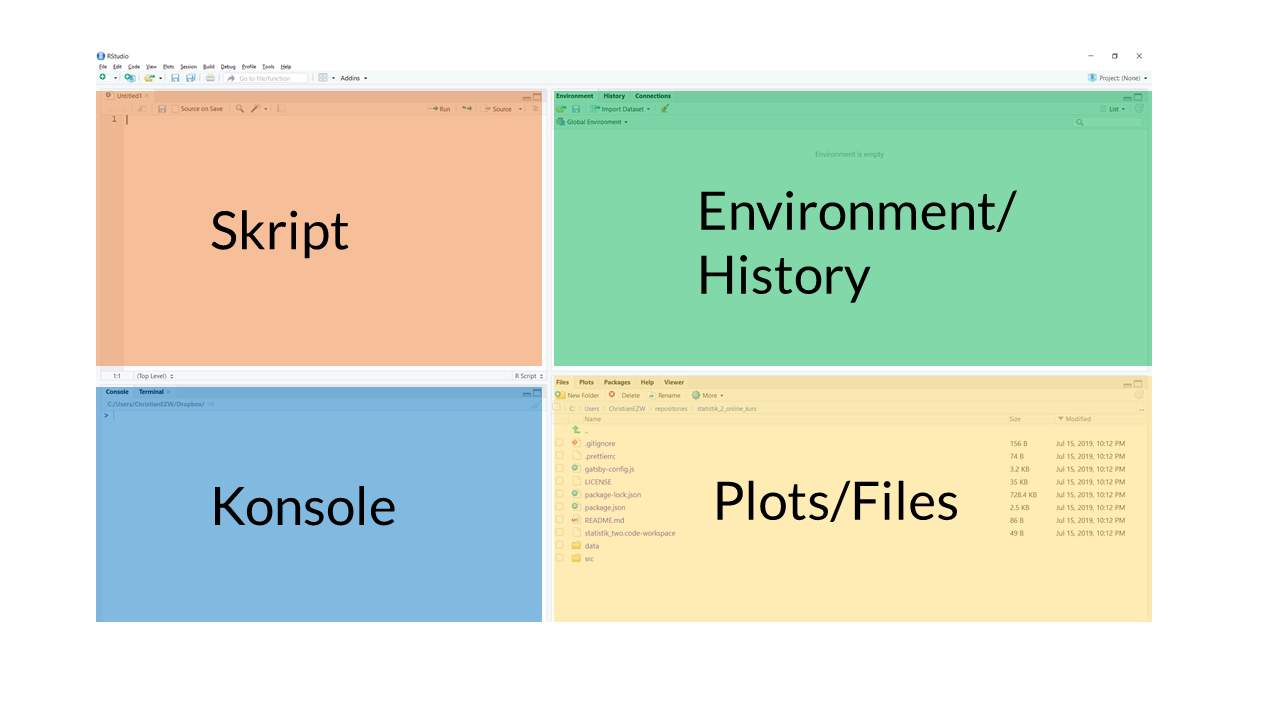
\includegraphics{images/02_grundlagen/rstudio_panels.jpg}

\begin{itemize}
\item
  Im Skript links oben findest du die R-Skripte. Dort speicherst du diejenigen Befehle, welche du auf jeden Fall speichern möchtest. Beispielsweise ein statistisches Verfahren, mit welchem du eine Hypothesen prüfst oder eine Visualisierung, die du erstellt hast.
\item
  In der Konsole links unten probierst du verschiedene Befehle aus. Die Konsole ist flüchtig und daher kein Ort, um dauerhaft Berechnungen zu sichern. Hierfür verwendest du am besten das Skript.
\item
  Das Environment und die History im Fenster rechts oben ist für diesen Kurs weniger relevant. Im Environment siehst du, auf welche Variablen und Daten du zugreifen kannst.
\item
  Rechts unten findest du den Output und die Plots/Visualisierungen. In der Regel schaust du hier deine Visualisierungen an, die du im Skript bzw. in der Konsole erstellst.
\end{itemize}

\hypertarget{befehle-aus-der-konsole-ausfuxfchren}{%
\subsection{Befehle aus der Konsole ausführen}\label{befehle-aus-der-konsole-ausfuxfchren}}

Befehle lassen sich sowohl in der Konsole als auch im Skript ausführen. Als Faustregel: Die Konsole dient dem Herumspielen mit den Daten, im Skript schreibst du alle Befehle auf, die du gerne behalten möchtest. Nehmen wir an, du möchtest die Zahl 5 mit der Zahl 8 addieren:

\begin{Shaded}
\begin{Highlighting}[]
\DecValTok{5} \SpecialCharTok{+} \DecValTok{8}
\end{Highlighting}
\end{Shaded}

\begin{verbatim}
## [1] 13
\end{verbatim}

Um den Befehl in der Konsole auszuführen, drückst du die \textbf{ENTER-Taste}

Anschließend erhältst du das Ergebnis der Berechnung. Um diesen Output aus der Konsole wieder zu entfernen, kannst du die Tastenkombination \textbf{STRG+L} verwenden. Hierdurch verschwindet der Output:

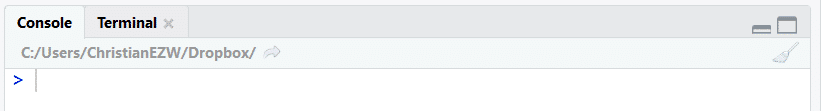
\includegraphics{images/02_grundlagen/console.png}

Wenn du eine Grafik erstellst (den Code musst du an dieser Stelle nicht verstehen), wird der Output in dem Plots Panel angezeigt, ohne dass du in der Konsole einen Output erhältst:

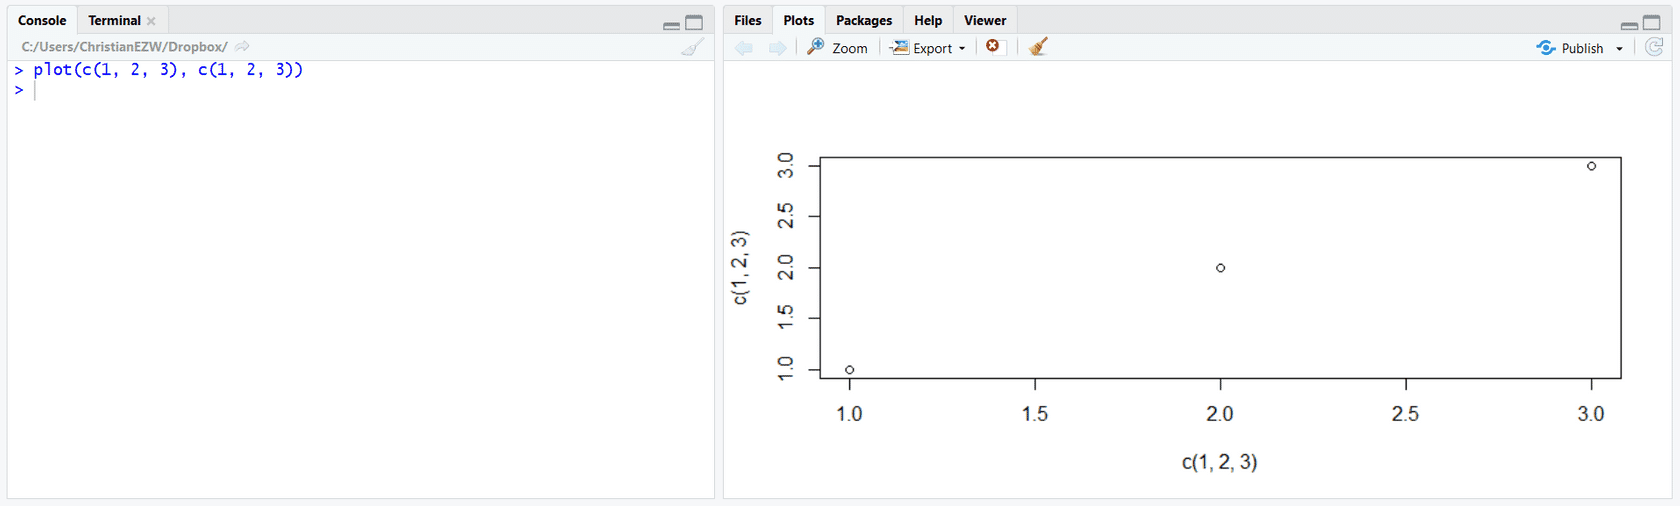
\includegraphics{images/02_grundlagen/plot.png}

\hypertarget{befehle-aus-dem-skript-ausfuxfchren}{%
\subsection{Befehle aus dem Skript ausführen}\label{befehle-aus-dem-skript-ausfuxfchren}}

Genau die gleichen Befehle kannst du aus einem Skript ausführen (Um ein neues Skript zu öffnen drücke \textbf{STRG + UMSCHALT + N} auf deiner Tastatur):

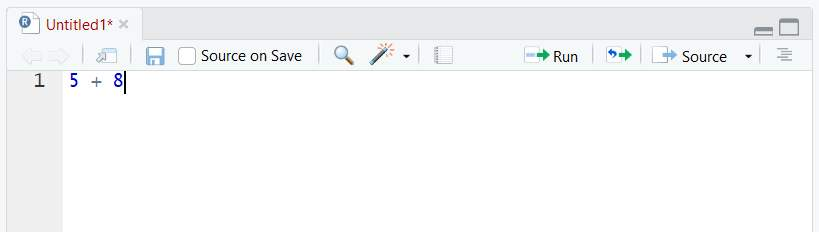
\includegraphics{images/02_grundlagen/befehle_skrip.jpg}

Um diesen Befehl auszuführen, musst du Deinen Cursor auf die jeweilige Zeile legen und \textbf{STRG+ENTER} drücken (für Mac-Nutzer: command + enter):

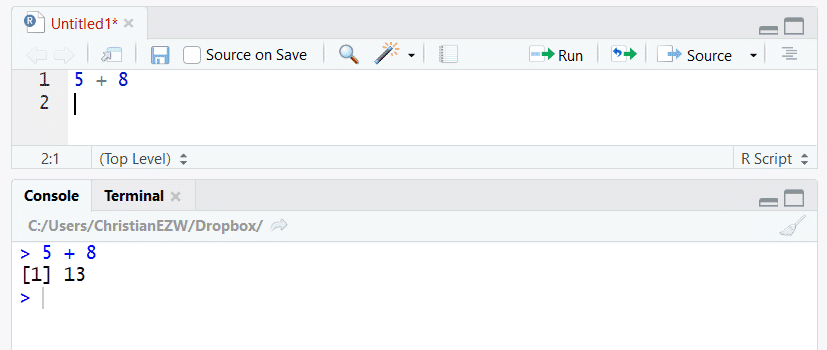
\includegraphics{images/02_grundlagen/befehle_skript1.png}

Wenn du ENTER-Taste nicht drückst, springt der Cursor in die nächste Zeile, ohne dass der Befehl ausgeführt wird. Alternativ kannst du die Zeile ausführen, indem du den Button Run drückst:

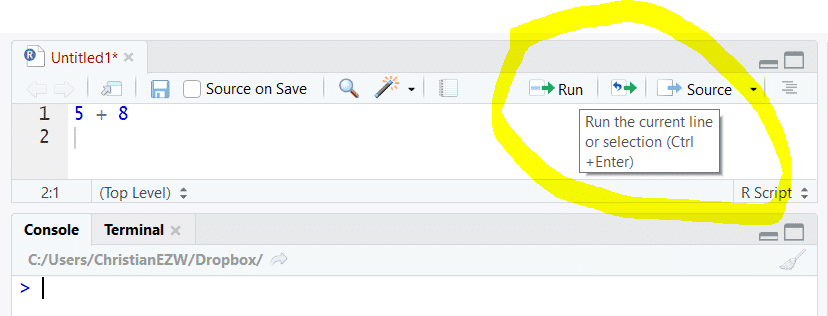
\includegraphics{images/02_grundlagen/run.png}

Um mehrere Zeilen ausführen, musst du mehrere Zeilen selektieren und STRG+ENTER drücken:

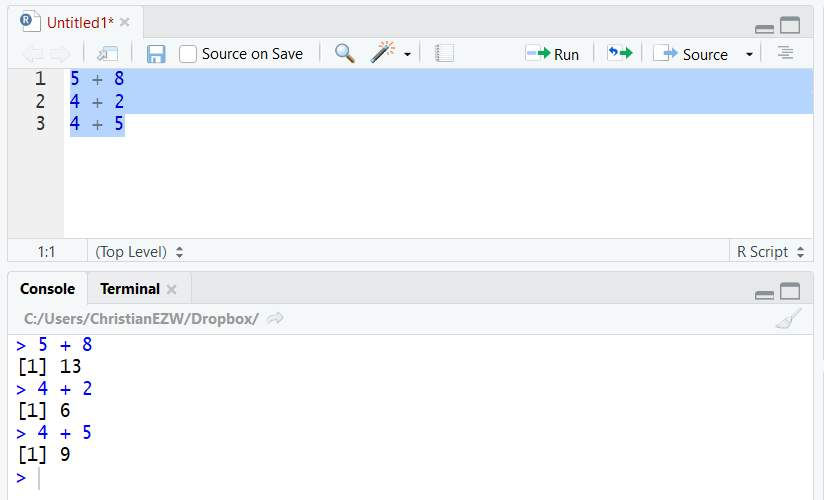
\includegraphics{images/02_grundlagen/multi_run.jpg}

\hypertarget{pakete-installieren-und-laden}{%
\subsection{Pakete installieren und laden}\label{pakete-installieren-und-laden}}

Ein Paket ist eine Sammlung an Funktionen und Daten, welche du gebündelt herunterladen kannst. Pakete erweitern die Funktionalität von R. R hat bereits viele Funktionen, die wir für die Datenanalyse verwenden können. Beispielsweise umfasst R die Funktion mean, mit der wir Mittelwerte aus einer Variablen berechnen können. Selbst wenn R hunderte Funktionen hat, die mit R mitgeliefert werden, brauchen wir häufig weitere Funktionen, um unsere Daten zu analysieren. Für diesen Kurs benötigen wir insbesondere Pakete, mit denen wir Daten analysieren, visualisieren und auswerten können. In diesem Kurs verwenden wir folgende Pakete:

\begin{itemize}
\item
  \href{https://rise.articulate.com/author/SHojwTyVccfVjJhG_D37L6cXrgxGbnca\#/author/details/anYDnxw9kjDldfma4gUcOvsHCpVUSe5-}{tidyverse}: Tidyverse umfasst eine Vielzahl an Paketen zur Analyse und Verarbeitung von Daten. Die Pakete haben eine einheitliche Philosophie und arbeiten reibungslos miteinander.
\item
  \href{https://cran.r-project.org/web/packages/jmv/index.html}{jmv \textgreater= 1.2.23}: jmv ist ein Paket, welches mit Jamovi zusammen arbeitet und uns ermöglicht, die Analysen, die wir in Jamovi umgesetzt haben, in R zu übertragen.
\item
  \href{https://github.com/sfirke/janitor}{janitor}: Viele Datensätze sind unstrukturiert und enthalten komplexe Variablennamen. Mit dem Paket janitor können wir diese bereinigen.
\item
  \href{https://github.com/r-lib/styler}{styler}: Mit styler können wir unseren Code so formatieren, dass er den Gestaltungsrichtlinien entspricht. Beispielsweise möchten wir nicht, dass eine Zeile Code länger als 80 Zeilen ist. Mit Hilfe von styler können wir solche Fehler durch einen Klick korrigieren.
\end{itemize}

Du kannst zu jeder Zeit in R-Studio sehen, welche Pakete installiert sind, indem du dir den Package Panel anschaust (rechts unten in R-Studio):

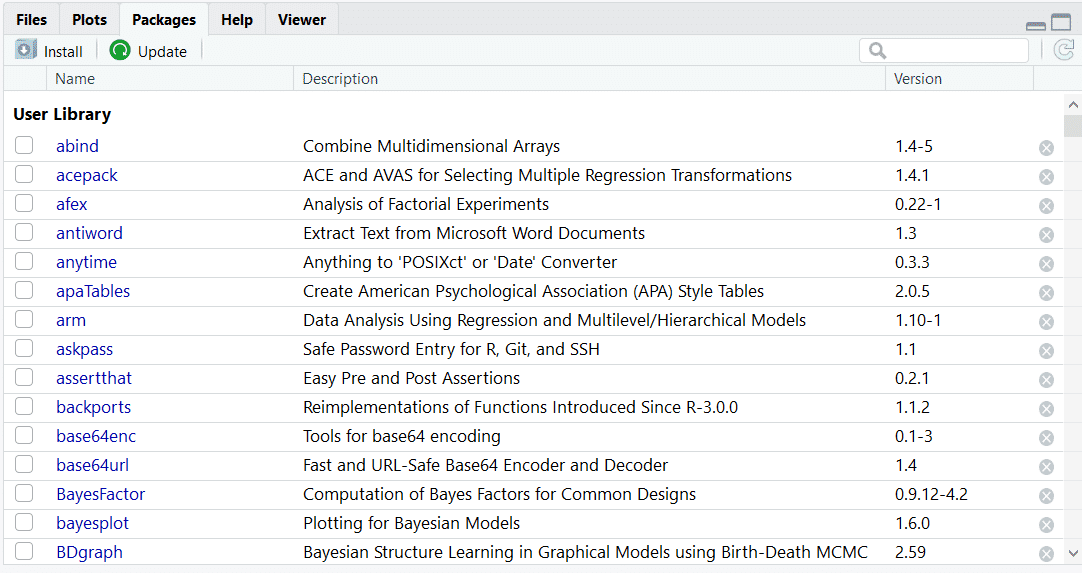
\includegraphics{images/02_grundlagen/pakete.png}

\hypertarget{pakete-intallieren}{%
\subsubsection{Pakete intallieren}\label{pakete-intallieren}}

Um Pakete zu installieren, kannst du in R-Studio auf Install unter dem Fenster Packages klicken:

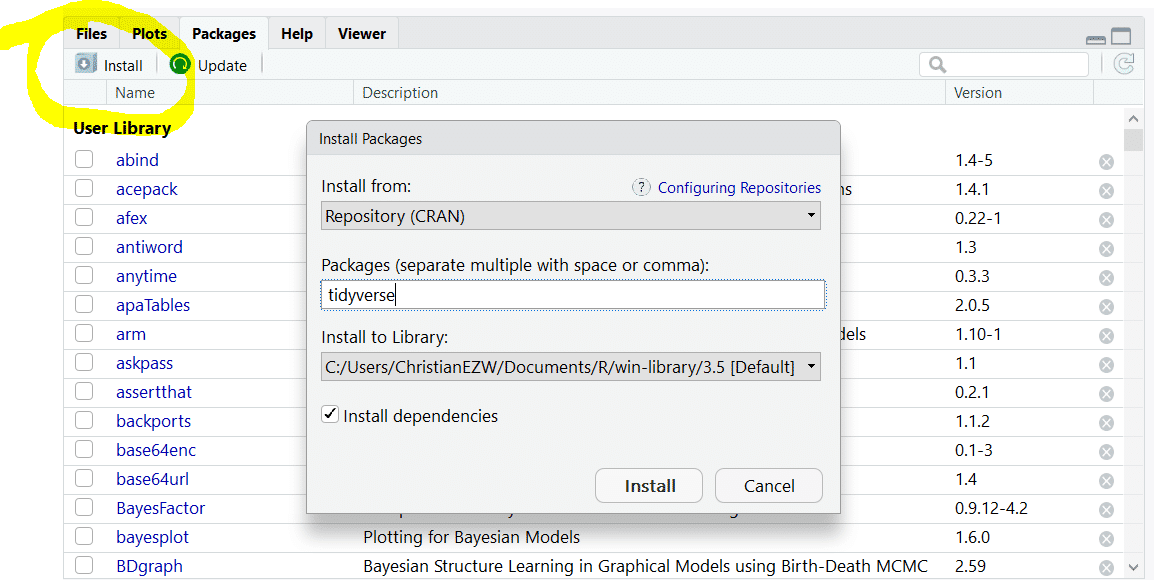
\includegraphics{images/02_grundlagen/install_pakete.png}

Trage zunächst das Paket unter Packages ein und drücke anschließend auf Install. Installiere sowohl tidyverse, janitor, jmv als auch styler. Alternativ kannst du direkt den Befehl in die Konsole eingeben, um die Pakete zu installieren (führe die Befehle am besten nacheinander aus):

\begin{verbatim}
>     install.packages("tidyverse")
>     # Dann
>     install.packages("janitor")
>     # Dann
>     install.packags("jmv")
>     # Dann
>     install.packags("styler")
\end{verbatim}

Prüfe anschließend, ob alle Pakete installiert wurden. Suche hierfür die Pakete in dem Panel Packages:

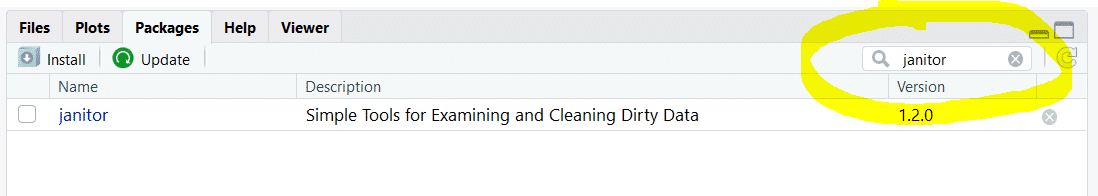
\includegraphics{images/02_grundlagen/pakete_check.png}

\hypertarget{pakete-laden}{%
\subsubsection{Pakete laden}\label{pakete-laden}}

Um die Funktionalität eines Paketes verwenden zu können, ist es mit der Installation nicht getan. Wir müssen die Pakete zusätzlich laden. Am besten lädst du die Pakete immer am Anfang deines R-Skripts, indem du folgende Befehl für jedes Paket eingibst:

\begin{verbatim}
>     library(tidyverse)
>     library(jmv)
\end{verbatim}

Um anschließend zu prüfen, welche Pakete gerade geladen sind, kannst du den Befehl sessionInfo() ausführen:~

\begin{verbatim}
> sessionInfo()
\end{verbatim}

TODO: hier ist die Schrift irgendwie anders (bei sessionInfo), aber ich kann es nicht umstellen.

\begin{verbatim}
>     R version 3.6.1 (2019-07-05)
>     ## Platform: x86_64-w64-mingw32/x64 (64-bit)
>     ## Running under: Windows 10 x64 (build 17763)
>     ## 
>     ## Matrix products: default
>     ## 
>     ## locale:
>     ## [1] LC_COLLATE=German_Germany.1252  LC_CTYPE=German_Germany.1252   
>     ## [3] LC_MONETARY=German_Germany.1252 LC_NUMERIC=C                   
>     ## [5] LC_TIME=German_Germany.1252    
>     ## 
>     ## attached base packages:
>     ## [1] stats     graphics  grDevices utils     datasets  methods   base     
>     ## 
>     ## other attached packages:
>     ##  [1] jmv_1.0.8       forcats_0.4.0   stringr_1.4.0   dplyr_0.8.3    
>     ##  [5] purrr_0.3.3     readr_1.3.1     tidyr_1.0.0     tibble_2.1.3   
>     ##  [9] ggplot2_3.2.1   tidyverse_1.2.1
>     ## 
>     ## loaded via a namespace (and not attached):
>     ##  [1] tidyselect_0.2.5 xfun_0.10        haven_2.1.1      lattice_0.20-38 
>     ##  [5] colorspace_1.4-1 vctrs_0.2.1      generics_0.0.2   htmltools_0.4.0 
>     ##  [9] yaml_2.2.0       rlang_0.4.2      pillar_1.4.3     glue_1.3.1      
>     ## [13] withr_2.1.2      modelr_0.1.5     readxl_1.3.1     jmvcore_1.0.8   
>     ## [17] lifecycle_0.1.0  munsell_0.5.0    gtable_0.3.0     cellranger_1.1.0
>     ## [21] rvest_0.3.4      evaluate_0.14    knitr_1.25       fansi_0.4.0     
>     ## [25] broom_0.5.2      Rcpp_1.0.3       backports_1.1.5  scales_1.1.0    
>     ## [29] jsonlite_1.6     rjson_0.2.20     hms_0.5.2        digest_0.6.23   
>     ## [33] stringi_1.4.3    bookdown_0.14    grid_3.6.1       cli_2.0.0       
>     ## [37] tools_3.6.1      magrittr_1.5     lazyeval_0.2.2   crayon_1.3.4    
>     ## [41] pkgconfig_2.0.3  zeallot_0.1.0    xml2_1.2.2       lubridate_1.7.4 
>     ## [45] assertthat_0.2.1 rmarkdown_1.16   httr_1.4.1       rstudioapi_0.10 
>     ## [49] R6_2.4.1         nlme_3.1-142     compiler_3.6.1
\end{verbatim}

Unter loaded via namespace kannst du erkennen, welche Pakete installiert sind, aber nicht geladen sind. Unter other attached packages siehst du, welche Pakete geladen sind, beispielsweise jmv. Erst nachdem ein Paket geladen ist, kannst du die Funktionen der Pakete verwenden. Wenn du R-Studio neu startest, muss jedes Paket immer neu geladen werden. Diesen Schritt vergisst man häufig, wodurch Fehler entstehen. Stelle daher immer sicher, dass du die nötigen Pakete lädst, bevor du Funktionen der Pakete verwendest. Um zu prüfen, aus welchem Paket eine Funktion stammt, setze ein Fragezeichen vor die Funktion (siehe nächstes Bild links oben). Anschließend siehst du die Dokumentation dieses Befehls in dem Panel Help:

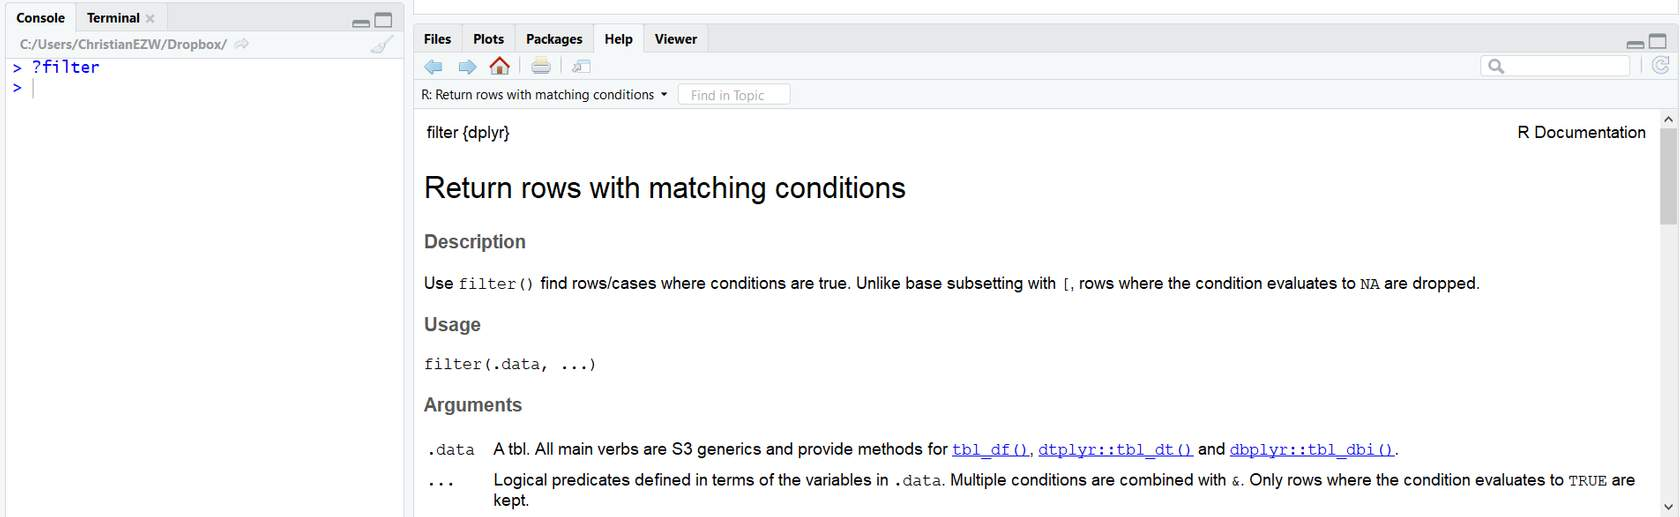
\includegraphics{images/02_grundlagen/panel_help.jpg}

\hypertarget{das-arbeitsverzeichnis}{%
\subsection{Das Arbeitsverzeichnis}\label{das-arbeitsverzeichnis}}

Wenn du R öffnest, legt R im Hintergrund immer einen Ordner fest, aus dem du alle Dateien importierst und exportierst. Diesen Ordner nennt man das Arbeitsverzeichnis. Du kannst dir das Arbeitsverzeichnis in R anzeigen lassen, indem du folgenden Befehl in der Konsole ausführst:

\begin{verbatim}
>     getwd()
\end{verbatim}

Als Output erhältst du das Verzeichnis des Ordners, welcher gerade als Arbeitsverzeichnis bestimmt ist:

\begin{verbatim}
>     [1] "C:/Users/Christian/Lehre/2020_ws_statistik_II"
\end{verbatim}

Solange du in R nicht mit \href{https://support.rstudio.com/hc/en-us/articles/200526207-Using-Projects}{Projekten} arbeitest, musst du wissen, wo das Arbeitsverzeichnis liegt, um Dateien zu importieren. Wenn du beispielsweise folgenden Befehl verwendest, um die Datei human\_resources.csv einzulesen, nimmt R automatisch an, dass sich diese Datei im Arbeitsverzeichnis befindet:

\begin{verbatim}
>     # Nehmen wir an, dass sich das Arbeitsverzeichnis 
>     # in folgendem Ordner befindet: 
>     #    C:/Users/Christian/Dropbox/Lehre
>     human_resources <- read_csv("human_resources.csv")
\end{verbatim}

Der Text zwischen den Anführungszeichen wird auch als relativer Pfad bezeichnet. Liegt die Datei beispielsweise einen Ordner über dem Arbeitsverzeichnis (in unserem Beispiel im Ordner Dropbox), verwenden wir zwei Punkte, um einen Ordner nach oben zu klettern:

\begin{verbatim}
>     # Nehmen wir an, dass sich das Arbeitsverzeichnis 
>     # in folgendem Ordner befindet: 
>     #    C:/Users/Christian/Dropbox/Lehre
>     human_resources <- read_csv("../human_resources.csv")
\end{verbatim}

Nun sucht R die Datei \emph{human\_resources.csv} im Ordner Dropbox. Die einfachste Methode, um allerdings eine Datei zu importieren, ist, das Arbeitsverzeichnis dort festzulegen, wo die Datei gespeichert ist. Dies können wir tun, indem wir den Shortcut \textbf{Ctrl+ UMSCHALT + H} in R-Studio ausführen. Danach öffnet sich ein Fenster, in dem wir das Arbeitsverzeichnis bestimmen können.

\hypertarget{datensuxe4tze-importieren}{%
\subsection{Datensätze importieren}\label{datensuxe4tze-importieren}}

In diesem Kurs arbeiten wir mit Daten, die in Tabellen angeordnet sind. Häufig liegen Daten als Excel-Dateien vor. Ein gängiges Format, um Daten zu speichern sind allerdings \href{https://de.wikipedia.org/wiki/CSV_(Dateiformat)}{CSV-Dateien}. CSV steht für Comma Seperated Values. Dies bedeutet, dass Werte in CSV-Dateien entweder durch ein Komma oder ein Semikolon getrennt sind. In folgendem Beispiel siehst du ein Datensatz mit drei Variablen, die in jeder Reihe durch ein Komma getrennt sind:

\begin{verbatim}
>     id,variable1,variable2
>     ku22su99,2,3
>     nn08se21,5,6
\end{verbatim}

TODO: Hier soll eigentlich eine Bildunterschrift hin mit ``Beispiel einer CSV-Datei''. Ich wusste nicht wie ich das einfüge, wenn es kein Bild ist.

Da CSV-Dateien ein sehr bekanntes Dateiformat für Daten sind, lassen sich CSV-Dateien sowohl in Excel, Jamovi, SPSS, als auch R importieren (\href{https://support.microsoft.com/de-de/office/importieren-oder-exportieren-von-textdateien-txt-oder-csv-5250ac4c-663c-47ce-937b-339e391393ba?ui=de-de\&rs=de-de\&ad=de}{Excel}, \href{https://www.youtube.com/watch?v=-imCiECplPo}{SPSS}, \href{https://www.youtube.com/watch?v=R0uE4LlHeac}{Jamovi}). Wir werden in diesem Modul mit dem Datensatz \emph{human\_resources.csv} arbeiten. Den Datensatz kannst du dir unter folgendem Link herunter laden:

TODO: Hier kommt eine Datei rein. Ich wusste nicht wie ich sie einfüge. human\_resources.csv

Eine CSV-Datei können wir in R importieren, indem wir die Datei in dem \emph{Panel Files} suchen und auf die Datei klicken. Klicke anschließend auf auf \emph{Import Dataset}:

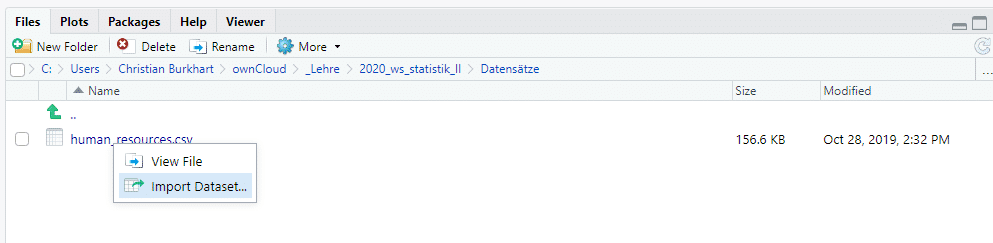
\includegraphics{images/02_grundlagen/csv_.png}

Anschließend siehst du ein neues Fenster, in welchem der Code angezeigt wird, mit dem wir die Daten importieren können. Kopiere am einfachsten die zweite Zeile des Code Preview (gelb markiert) und drücke dann auf Cancel.~

Falls die Daten nicht sauber in Spalten angeordnet sind, kannst du unter dem Reiter \emph{Delimiter} die Trennzeichen ändern. Im folgenden Beispiel sind die Trennzeichen in der CSV-Datei Kommas.

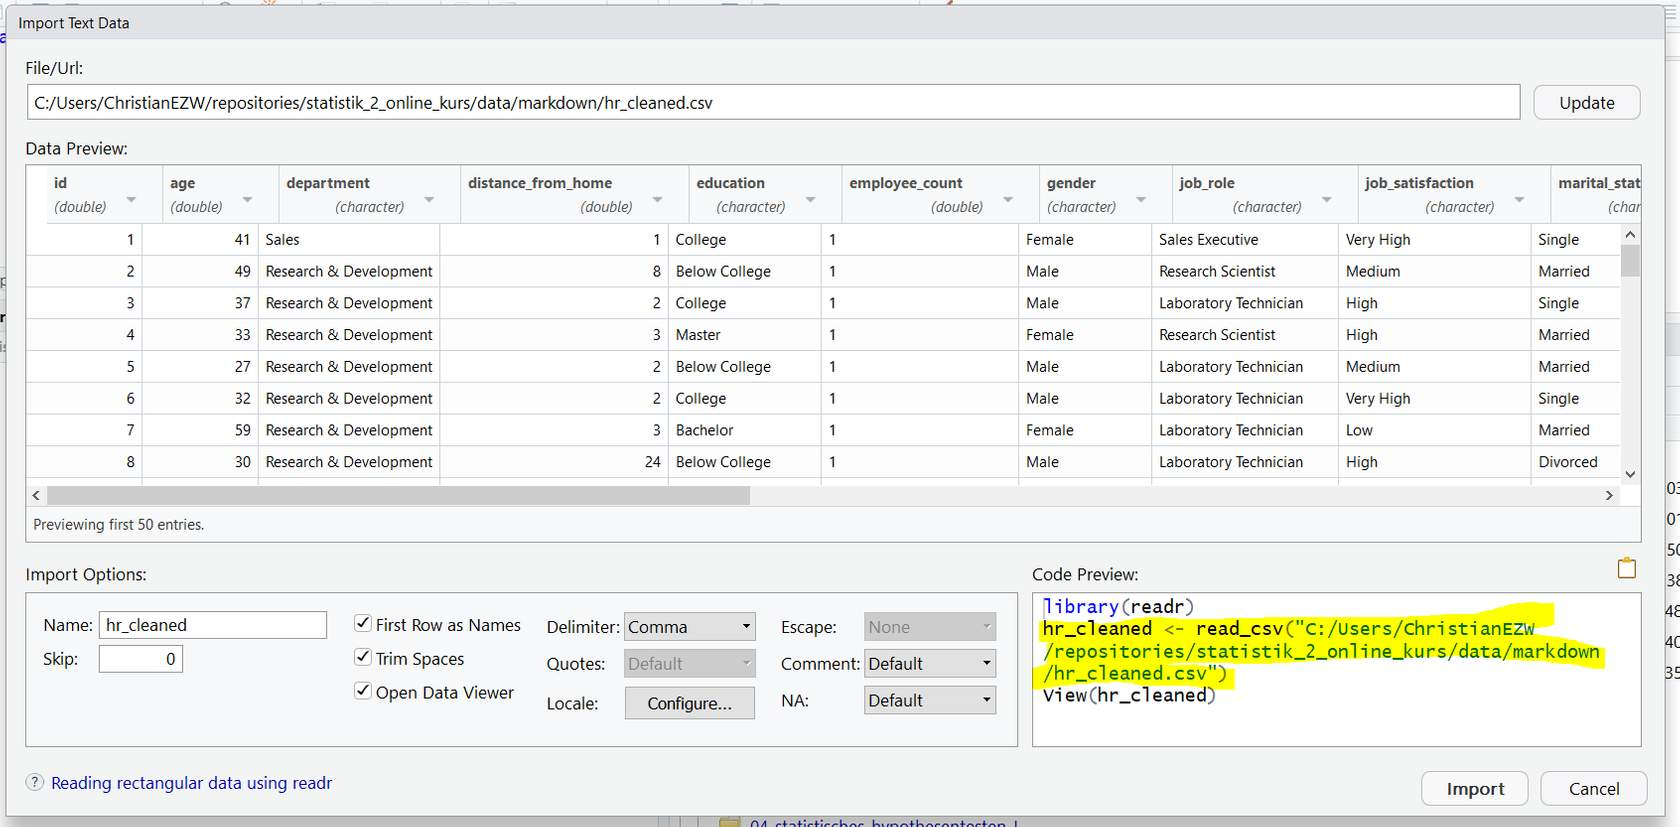
\includegraphics{images/02_grundlagen/table.jpg}

Diesen kopierten Code fügst du in dein R-Skript ein. Achte darauf, dass du vorher das Paket tidyverse lädst:~

\begin{figure}
\centering
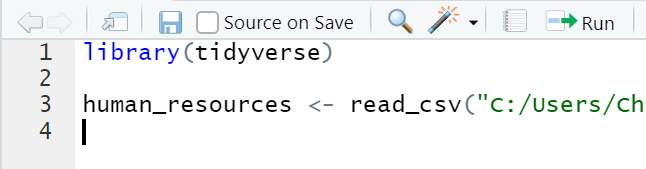
\includegraphics{images/02_grundlagen/load_dataset.jpg}
\caption{Beispiel für das Laden eines Datensatzes mit dem Paket tidyverse}
\end{figure}

Im nächsten Schritt liest du den Datensatz ein, indem du den Befehl ausführst:

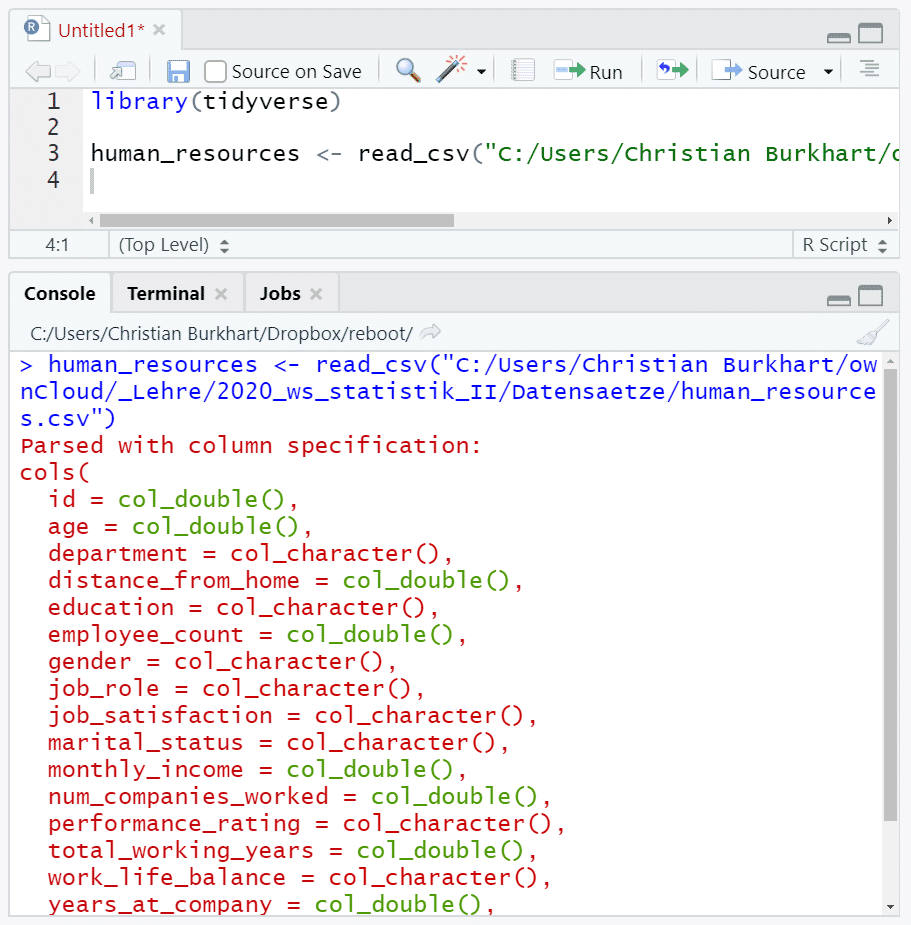
\includegraphics{images/02_grundlagen/load_data1.png}

Die rote Schrift hat keine Bedeutung. Sie zeigt an, welche Variablen der Datensatz umfasst. Um zu prüfen, ob der Datensatz in der Variable gespeichert wurde, gib den Datensatz in der Konsole aus:

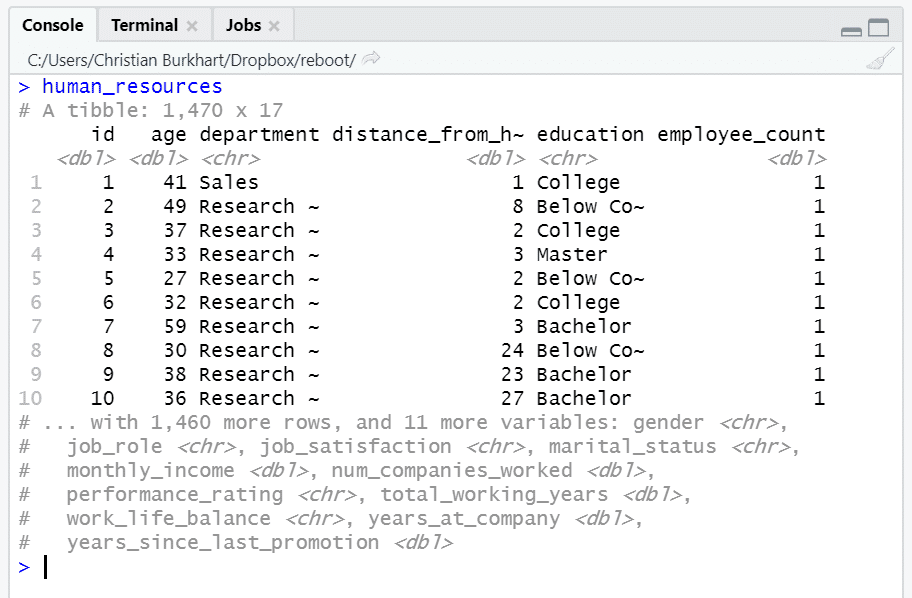
\includegraphics{images/02_grundlagen/enviroment.png}

Gleichzeitig kannst du im Panel Environment sehen, ob dein Datensatz geladen wurde:

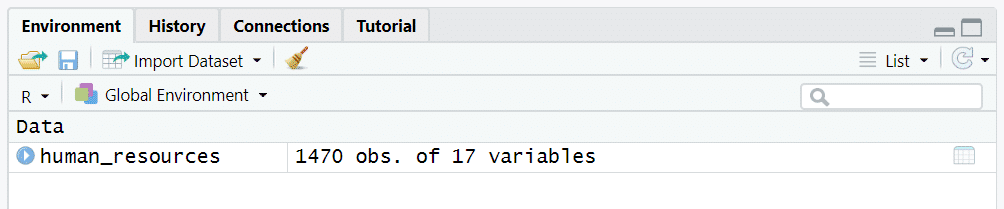
\includegraphics{images/02_grundlagen/environment1.png}

Der Output zeigt uns an, dass der Datensatz 1470 Reihen und 17 Variablen hat.

\hypertarget{grundlegende-operatoren-in-r}{%
\subsection{Grundlegende Operatoren in R}\label{grundlegende-operatoren-in-r}}

\hypertarget{rechenoperationen}{%
\subsubsection{Rechenoperationen}\label{rechenoperationen}}

R umfasst die typischen Rechenoperatoren, die du aus der Schule kennst. Du kannst mit R Plus, Minus oder Geteilt rechnen.

Zahlen voneinander teilen:

\begin{Shaded}
\begin{Highlighting}[]
\DecValTok{3} \SpecialCharTok{/} \DecValTok{9}
\end{Highlighting}
\end{Shaded}

\begin{verbatim}
## [1] 0.3333333
\end{verbatim}

Das Produkt zweier Zahlen berechnen:

\begin{Shaded}
\begin{Highlighting}[]
\DecValTok{3} \SpecialCharTok{*} \DecValTok{4}
\end{Highlighting}
\end{Shaded}

\begin{verbatim}
## [1] 12
\end{verbatim}

Zwei Zahlen miteinander addieren:

\begin{Shaded}
\begin{Highlighting}[]
\DecValTok{3} \SpecialCharTok{+} \DecValTok{4} 
\end{Highlighting}
\end{Shaded}

\begin{verbatim}
## [1] 7
\end{verbatim}

Die Zeichen +, -, / oder * nennen wir Operatoren. Operatoren sind nichts anderes als besondere Symbole, die eine bestimmte Aufgabe haben. Zum Beispiel hat der Operator + die Aufgabe, zwei Zahlen zu addieren. Wir können ebenso mehrere Operatoren miteinander verschachteln:

\begin{Shaded}
\begin{Highlighting}[]
\NormalTok{(}\DecValTok{3} \SpecialCharTok{/} \DecValTok{9}\NormalTok{) }\SpecialCharTok{*} \DecValTok{4} \SpecialCharTok{+} \DecValTok{3}
\end{Highlighting}
\end{Shaded}

\begin{verbatim}
## [1] 4.333333
\end{verbatim}

\hypertarget{der-zuordnungsoperator}{%
\subsubsection{Der Zuordnungsoperator}\label{der-zuordnungsoperator}}

Der Zuordnungsoperator \textless- wird verwendet, um Variablen zu kreiieren. Variablen kannst du dir wie Boxen bei einem Umzug vorstellen, die etwas enthalten. Jede Box bekommt ein Label, hier einen Variablennamen. Was in der Box steckt, kannst du erfahren, indem du die Box aufmachst, bzw. dir die Variable in R ausgeben lässt. Erstellen wir hierzu eine neue Variable mit dem Namen sum\_score:

\begin{verbatim}
>     sum_score <- 3 + 4
\end{verbatim}

Jede Variable umfasst drei Elemente:

\begin{enumerate}
\def\labelenumi{\arabic{enumi}.}
\item
  \textbf{Der Variablenname}: sum\_score beispielsweise. Dieser Name ist willkürlich. Er sollte nicht mit einer Zahl beginnen und kleingeschrieben sein. Trenne mehrere Wörter am besten mit einem Unterstrich (z.B. sum\_score).
\item
  \textbf{Der Zuordnungsoperator \textless-:} Achte darauf, dass vor dem \textless{} und hinter dem - ein Leerzeichen steht. Ebenso sollte zwischen Operatoren ein Leerzeichen stehen. Falsch: sum\_score\textless-3+4, falsch: sum\_score \textless- 3+4, richtig: sum\_score \textless- 3 + 4.
\item
  \textbf{Der Inhalt der Variable:} 3 + 4. Der Inhalt kann im Prinzip alles sein: Text: ``Hallo'', ein Datensatz: read\_csv(\ldots) oder der Output einer Funktion: mean(c(1, 3, 4))
\end{enumerate}

Wenn du eine Variable erstellst, passiert zunächst nichts. R speichert intern das Produkt in der Variable sum\_score. Um das Ergebnis der Berechnung zu sehen, führe die Variable in R aus:

\begin{verbatim}
>     sum_score

>     ## [1] 7
\end{verbatim}

Variablennamen sollten immer so geschrieben sein, dass man weiß, was in der Variable steckt:

\begin{verbatim}
>     x <- 3 + 2 # schlecht
>     summe_zahlen <- 3 + 2 # besser
\end{verbatim}

Trenne einzelne Wörter in der Variable mit einem Unterstrich:

\begin{verbatim}
>     my_age <- 24  # gut
>
>     my.age <- 24 # schlecht
>     my-age <- 24 # schlecht
>     my/age <- 24 # schlecht
\end{verbatim}

Schreibe Variablen am besten alle Buchstaben des Variablennamen in Kleinschreibung:

\begin{verbatim}
>     my_age <- 24
>     # nicht:
>     My_age <- 24
\end{verbatim}

Variablen sollten exakt angegeben werden. Kleinste Fehler führen zu Fehlern. Zum Beispiel macht die Groß- oder Kleinschreibung einen Unterschied:

\begin{verbatim}
>     > my_age <- 24
>     > My_age
>     Error: object 'My_age' not found
\end{verbatim}

\hypertarget{der-operator}{%
\subsubsection{Der == Operator}\label{der-operator}}

Wir können ebenso prüfen, ob zwei Werte gleich sind, indem wir den == Operator verwenden:

\begin{Shaded}
\begin{Highlighting}[]
\DecValTok{3} \SpecialCharTok{==} \DecValTok{4}
\end{Highlighting}
\end{Shaded}

\begin{verbatim}
## [1] FALSE
\end{verbatim}

Oder:

\begin{Shaded}
\begin{Highlighting}[]
\DecValTok{3} \SpecialCharTok{==} \DecValTok{3}
\end{Highlighting}
\end{Shaded}

\begin{verbatim}
## [1] TRUE
\end{verbatim}

Oder:

\begin{Shaded}
\begin{Highlighting}[]
\DecValTok{3} \SpecialCharTok{==} \DecValTok{1} \SpecialCharTok{+} \DecValTok{2}
\end{Highlighting}
\end{Shaded}

\begin{verbatim}
## [1] TRUE
\end{verbatim}

Später werden wir diesen Operator verwenden, um Reihen in einem Datensatz zu filtern. Eine volle Liste der restlichen Operatoren findest du \href{https://www.statmethods.net/management/operators.html}{hier}.

\hypertarget{funktionen}{%
\subsection{Funktionen}\label{funktionen}}

Jede Programmiersprache ist nur so umfangreich, wie viele Funktionen sie hat. Funktionen werden von Menschen geschrieben, deren Ziel es ist, verschiedenste Berechnungen zu automatisieren. Gib zum Beispiel einmal in deine Konsole nur die Funktion mean ein. Was du erhältst ist der Beginn einer Funktion, die Menschen für die Programmiersprache R geschrieben haben. Funktionen haben immer den gleichen Aufbau:

\begin{verbatim}
>     function_name(argument1 = value1, argument2 = value2)
\end{verbatim}

\begin{itemize}
\item
  \textbf{function\_name}: Dies ist der Name der Funktion. Auch dieser ist wie bei Variablen willkürlich gewählt.
\item
  \textbf{argument1}: Funktionen haben immer Argumente. Ein Argument besagt, welche Objekte in eine Funktion gespeist werden. Stell dir Funktionen wie eine Fabrik vor, die etwas herstellt. Jede Fabrik benötigt Rohmaterial mit dem Produkte erzeugt werden. Argumente sind äquivalent zu Rohmaterialien. Sie werden in die Funktion gespeist und in der Funktion verarbeitet.
\item
  \textbf{value1}: Jedes dieser Rohmaterialien hat bestimmte Werte. Beispielsweise kann value1 eine Zahl (3) oder ein Text sein (``Hallo''). Wir werden später andere Datentypen kennen lernen, die ebenso in Funktionen gespeist werden können (z.B. Vektoren oder Dataframes - mehr dazu gleich).
\end{itemize}

Beispielsweise umfasst R die Funktion sqrt mit der wir die Wurzel einer Zahl berechnen können:

\begin{Shaded}
\begin{Highlighting}[]
\FunctionTok{sqrt}\NormalTok{(}\DecValTok{9}\NormalTok{)}
\end{Highlighting}
\end{Shaded}

\begin{verbatim}
## [1] 3
\end{verbatim}

Mit Hilfe des ? Zeichens können wir die Funktion näher betrachten und uns ansehen, welche Argumente eine Funktion annimmt:

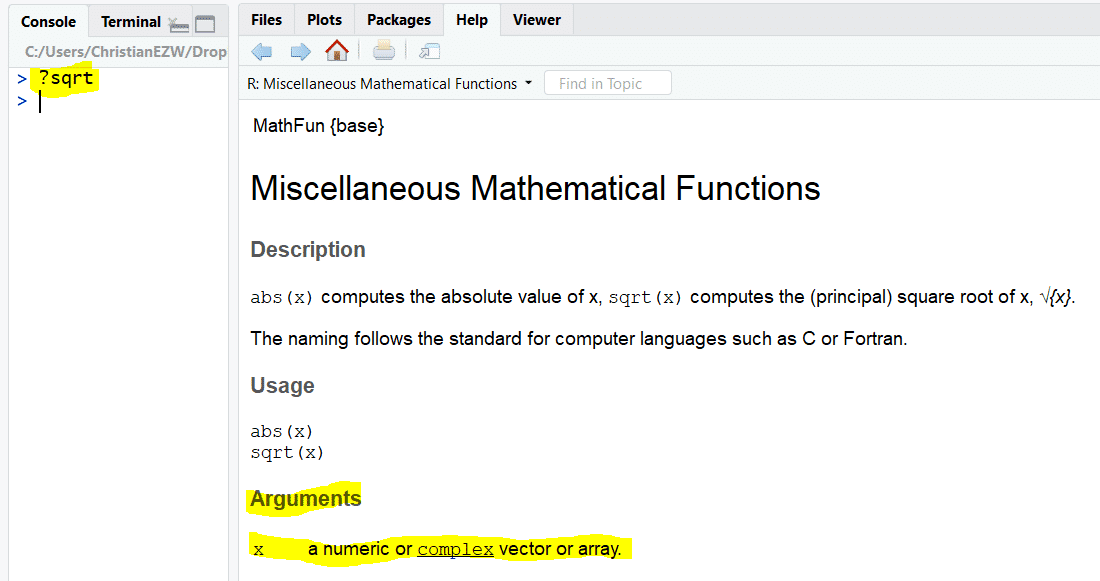
\includegraphics{images/02_grundlagen/funktion.png}

Die Funktion sqrt hat demnach nur ein Argument mit dem Namen x. x kann sowohl eine einzelne Zahl als auch mehrere Zahlen sein. Wir müssen das Argument nicht immer angeben. Wir hätten die Funktion daher auch so formulieren können:

\begin{Shaded}
\begin{Highlighting}[]
\FunctionTok{sqrt}\NormalTok{(}\AttributeTok{x =} \DecValTok{9}\NormalTok{)}
\end{Highlighting}
\end{Shaded}

\begin{verbatim}
## [1] 3
\end{verbatim}

Achte darauf, dass jede Funktion mit einer Klammer schließt. Tust du dies nicht, denkt R, dass dein Befehl noch nicht zu Ende ist und zeigt Dir dies mit einem + an:

\begin{verbatim}
>     > sqrt(9
>     +
\end{verbatim}

Eine andere Funktion heißt sum. Mit sum kannst du mehrere Zahlen miteinander addieren:

\begin{Shaded}
\begin{Highlighting}[]
\FunctionTok{sum}\NormalTok{(}\DecValTok{3}\NormalTok{, }\DecValTok{4}\NormalTok{, }\DecValTok{5}\NormalTok{)}
\end{Highlighting}
\end{Shaded}

\begin{verbatim}
## [1] 12
\end{verbatim}

Wenn du dir die Funktion unter der Hilfe mit ?sum anschaust, erkennst du, dass die Funktion unendlich viele Argumente hat. Dies wird mit einem \ldots{} gekennzeichnet:

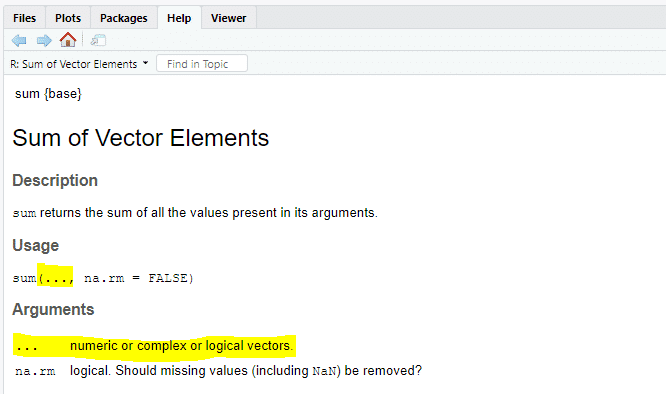
\includegraphics{images/02_grundlagen/sum.png}

Wir könnten daher ebenso die Summe von fünf Zahlen zusammen rechnen:

\begin{Shaded}
\begin{Highlighting}[]
\FunctionTok{sum}\NormalTok{(}\DecValTok{1}\NormalTok{, }\DecValTok{2}\NormalTok{, }\DecValTok{3}\NormalTok{, }\DecValTok{4}\NormalTok{, }\DecValTok{5}\NormalTok{)}
\end{Highlighting}
\end{Shaded}

\begin{verbatim}
## [1] 15
\end{verbatim}

Lade als nächstes das Paket tidyverse (library(tidyverse)). Das Paket tidyverse umfasst die Funktion select. Mit Hilfe von select werden wir später Variablen aus einem Datensatz selektieren. Wenn du dir die Dokumentation der Funktion mit Hilfe von ?select anschaust, erkennst du, dass die Funktion mehrere Argumente hat:

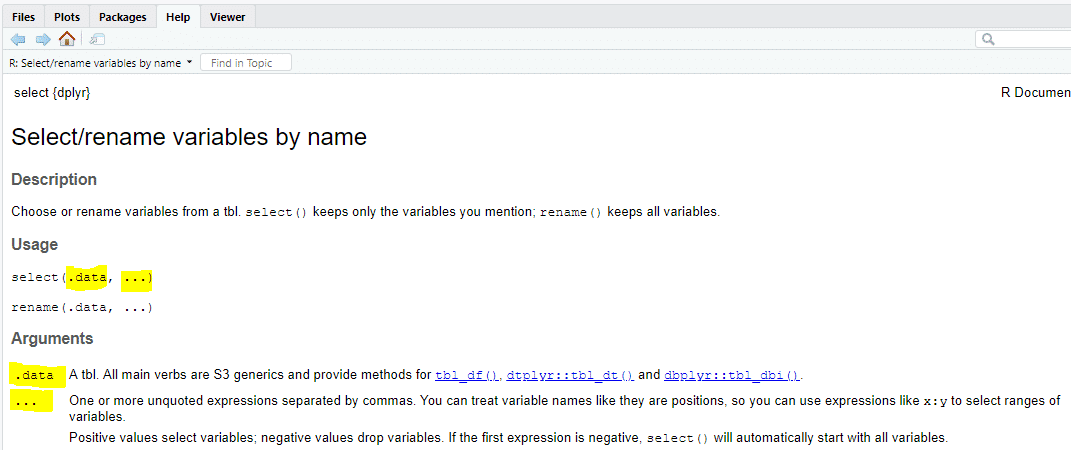
\includegraphics{images/02_grundlagen/select.png}

Das erste Argument heißt .data. Hierfür fügen wir später den Datensatz ein. Das zweite Argument hat keinen expliziten Namen, sondern umfasst eine mit Komma getrennte Liste an Variablennamen. Schauen wir uns ein Beispiel an. Hierfür laden wir zunächst das Paket tidyverse und den Datensatz \emph{human\_resources}:

\begin{verbatim}
>     library(tidyverse)
>     human_resources <- read_csv("human_resources.csv")
\end{verbatim}

Anschließend können wir die Funktion select ausführen, um verschiede Variablen aus dem Datensatz zu nehmen (Um zu sehen, welche Variablen im Datensatz stecken, gebe colnames(human\_resources) in die Konsole ein):

\begin{verbatim}
>     select(.data = human_resources, id, age)

>     ## # A tibble: 1,470 x 2
>     ##       id   age
>     ##    <dbl> <dbl>
>     ##  1     1    41
>     ##  2     2    49
>     ##  3     3    37
>     ##  4     4    33
>     ##  5     5    27
>     ##  6     6    32
>     ##  7     7    59
>     ##  8     8    30
>     ##  9     9    38
>     ## 10    10    36
>     ## # … with 1,460 more rows
\end{verbatim}

Du erkennst das erste Argument .data, in welches wir den Datensatz einfügen. Zusätzlich geben wir mehrere Variablennamen ein, indem wir die Variablennamen durch ein Komma trennen. Wir hätten ebenso die Argumente umdrehen können:

\begin{verbatim}
>     select(id, age, .data = human_resources)

>     ## # A tibble: 1,470 x 2
>     ##       id   age
>     ##    <dbl> <dbl>
>     ##  1     1    41
>     ##  2     2    49
>     ##  3     3    37
>     ##  4     4    33
>     ##  5     5    27
>     ##  6     6    32
>     ##  7     7    59
>     ##  8     8    30
>     ##  9     9    38
>     ## 10    10    36
>     ## # … with 1,460 more rows
\end{verbatim}

Generell ist es allerdings ratsam, die Reihenfolge der Argumente beizubehalten. Wenn wir dies tun, können wir die Namen der Argumente ignorieren:

\begin{verbatim}
>     select(human_resources, id, age)
\end{verbatim}

Versuchen wir nochmal von diesem Beispiel zu abstrahieren. Funktionen haben einen Namen und eine umgebende Klammer:

\begin{verbatim}
>     function_name()
\end{verbatim}

Fasst alle Funktionen haben Argumente. Die Anzahl der Argumente ist abhängig von der Funktion. Hier siehst du das Schema einer Funktion mit zwei Argumenten:

\begin{verbatim}
>     function_name(argument1 = value1, argument2 = value2)
\end{verbatim}

Die Reihenfolge der Argumente ist egal, solange wir die Argumente explizit benennen:

\begin{verbatim}
>     function_name(argument2 = value2, argument1 = value1)
\end{verbatim}

Bennenen wir die Argumente nicht, müssen wir die Reihenfolge beachten, die in der Funktion (siehe ?function\_name) vorgegeben ist:

\begin{verbatim}
>     function_name(value1, value2)
\end{verbatim}

\hypertarget{grundlegende-funktionen-in-r}{%
\subsection{Grundlegende Funktionen in R}\label{grundlegende-funktionen-in-r}}

Es gibt ein paar wenige Befehle, die du immer wieder in R benötigst. Wir werden die Befehle anhand des Datensatzes \emph{human\_resources.csv} kennen lernen, den du hier herunterladen kannst:

TODO: Einfügen Datei: human\_resources.csv

Zunächst müssen wir tidyverse laden und den Datensatz importieren:

\begin{verbatim}
>     library(tidyverse)
>     human_resources <- read_csv("human_resources.csv")
\end{verbatim}

Mit \href{https://www.rdocumentation.org/packages/utils/versions/3.6.1/topics/View}{View}kannst du Dir den Datensatz in einem Excel-ähnlichen Format betrachten:

\begin{verbatim}
>     View(human_resources)
\end{verbatim}

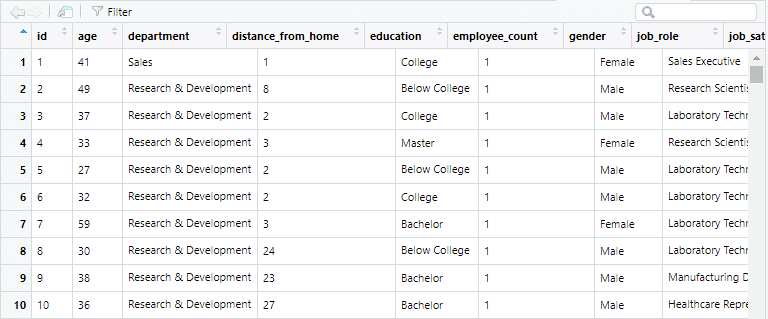
\includegraphics{images/02_grundlagen/view_hr.png}

Du kannst dir die Variablennamen mit der Funktion colnames ausgeben lassen:

\begin{verbatim}
>     colnames(human_resources)

>     ##  [1] "id"                         "age"                       
>     ##  [3] "department"                 "distance_from_home"        
>     ##  [5] "education"                  "employee_count"            
>     ##  [7] "gender"                     "job_role"                  
>     ##  [9] "job_satisfaction"           "marital_status"            
>     ## [11] "monthly_income"             "num_companies_worked"      
>     ## [13] "performance_rating"         "total_working_years"       
>     ## [15] "work_life_balance"          "years_at_company"          
>     ## [17] "years_since_last_promotion"
\end{verbatim}

Manchmal möchte man wissen, wie viele Reihen in einem Datensatz stecken. Hierfür kannst du die Funktion \href{https://www.rdocumentation.org/packages/base/versions/3.6.1/topics/nrow}{nrow}verwenden:

\begin{verbatim}
>     nrow(human_resources)

>     ## [1] 1470
\end{verbatim}

Genausogut lassen sich die Anzahl der Variablen (bzw. Spalten) in einem Datensatz mit der Funktion \href{https://www.rdocumentation.org/packages/base/versions/3.6.1/topics/nrow}{ncol}ausgeben lassen:

\begin{verbatim}
>     ncol(human_resources)

>     ## [1] 17
\end{verbatim}

Zuletzt benötigen wir noch die Funktion head. Mithilfe von head können wir uns die ersten Reihen eines Datensatzes ansehen:

\begin{verbatim}
>     head(human_resources)

>     ## # A tibble: 6 x 17
>     ##      id   age department distance_from_h… education employee_count gender
>     ##   <dbl> <dbl> <chr>                 <dbl> <chr>              <dbl> <chr> 
>     ## 1     1    41 Sales                     1 College                1 Female
>     ## 2     2    49 Research …                8 Below Co…              1 Male  
>     ## 3     3    37 Research …                2 College                1 Male  
>     ## 4     4    33 Research …                3 Master                 1 Female
>     ## 5     5    27 Research …                2 Below Co…              1 Male  
>     ## 6     6    32 Research …                2 College                1 Male  
>     ## # … with 10 more variables: job_role <chr>, job_satisfaction <chr>,
>     ## #   marital_status <chr>, monthly_income <dbl>,
>     ## #   num_companies_worked <dbl>, performance_rating <chr>,
>     ## #   total_working_years <dbl>, work_life_balance <chr>,
>     ## #   years_at_company <dbl>, years_since_last_promotion <dbl>
\end{verbatim}

\hypertarget{daten-exportieren}{%
\subsubsection{Daten exportieren}\label{daten-exportieren}}

Wenn wir Daten importieren möchten, wollen wir sie auch exportieren können. Wir werden in diesem Kurs mehrmals Daten bereinigen und verändern und möchten diese Daten anschließend wieder in einer CSV-Datei speichern. Hierfür benutzen wir die \href{https://readr.tidyverse.org/reference/write_delim.html}{\emph{write\_csv}}Funktion. Die Funktion \emph{write\_csv} hat zwei wichtige Argumente:

\begin{quote}
Achte darauf, dass du die Funktion nur verwenden kannst, wenn du das Paket tidyverse geladen hast.
\end{quote}

\begin{verbatim}
 write_csv(x, path)
\end{verbatim}

\begin{itemize}
\item
  x steht für den Datensatz, den wir der Funktion überführen.
\item
  path steht für den Dateinamen in denen wir die Datei speichern. Achte darauf, diesen Pfad immer mit Anführungsstrichen " zu umrunden.

  write\_csv(NAME\_GEREINIGER\_DATENSATZ, ``datensatz\_gereinigt.csv'')
\end{itemize}

\begin{quote}
R speichert die Datei immer in das aktuelle Arbeitsverzeichnis. Diese kannst du verändern, indem du mit dem Shortcut STRG + Umschalt + H (für Mac COMMAND + Umschalt + H) das Arbeitsverzeichnis wechselt. In diesen Ordner wird die Datei anschließend gespeichert.
\end{quote}

\hypertarget{grundlagen-tidyverse}{%
\section{Grundlagen tidyverse}\label{grundlagen-tidyverse}}

\hypertarget{statistisches-hypothesentesten}{%
\chapter{Statistisches Hypothesentesten}\label{statistisches-hypothesentesten}}

We describe our methods in this chapter.

\hypertarget{was-sind-p-werte}{%
\section{Was sind p-Werte?}\label{was-sind-p-werte}}

\hypertarget{effektgruxf6uxdfen-einfuxfchren}{%
\section{Effektgrößen einführen}\label{effektgruxf6uxdfen-einfuxfchren}}

Das ist ein Quatschtext.

\hypertarget{hallo-christian}{%
\chapter{Hallo Christian}\label{hallo-christian}}

\hypertarget{ich-bin-clarissa}{%
\section{Ich bin Clarissa}\label{ich-bin-clarissa}}

\begin{itemize}
\tightlist
\item
  Item2
\item
  Item 3
\end{itemize}

\href{www.zeit.de}{link}

Wohnung \textbf{Herd} \emph{Text}

\begin{Shaded}
\begin{Highlighting}[]
\NormalTok{xy }\OtherTok{\textless{}{-}} \DecValTok{3} 
\end{Highlighting}
\end{Shaded}

\begin{Shaded}
\begin{Highlighting}[]
\NormalTok{xy }\SpecialCharTok{+} \DecValTok{5}
\end{Highlighting}
\end{Shaded}

\begin{verbatim}
## [1] 8
\end{verbatim}

\hypertarget{statistische-modellierung}{%
\chapter{Statistische Modellierung}\label{statistische-modellierung}}

Vom allgemeinen linearen Modell sprechen

\hypertarget{konfidenzintervalle}{%
\section{Konfidenzintervalle}\label{konfidenzintervalle}}

anhand der Parameter erklären und was sie bedeuten

\begin{itemize}
\tightlist
\item
  \url{https://thenewstatistics.com/itns/2020/07/04/3-easy-ways-to-obtain-cohens-d-and-its-ci/}
\item
  \url{http://www.tqmp.org/RegularArticles/vol14-4/p242/p242.pdf}
\end{itemize}

\hypertarget{einfache-lineare-regression}{%
\chapter{Einfache lineare Regression}\label{einfache-lineare-regression}}

We have finished a nice book.

\hypertarget{weitere-ressourcen}{%
\section{Weitere Ressourcen}\label{weitere-ressourcen}}

\begin{itemize}
\tightlist
\item
  \url{https://www.r-bloggers.com/2020/12/robust-regression/}
\end{itemize}

\hypertarget{multiple-lineare-regression}{%
\chapter{Multiple lineare Regression}\label{multiple-lineare-regression}}

We have finished a nice book.

\hypertarget{einfaktorielle-varianzanalyse}{%
\chapter{Einfaktorielle Varianzanalyse}\label{einfaktorielle-varianzanalyse}}

We have finished a nice book.

\begin{itemize}
\tightlist
\item
  Welch-Test nicht vergessen
\end{itemize}

\hypertarget{mehrfaktorielle-varianzanalyse}{%
\chapter{Mehrfaktorielle Varianzanalyse}\label{mehrfaktorielle-varianzanalyse}}

We have finished a nice book.

\hypertarget{ancova}{%
\chapter{ANCOVA}\label{ancova}}

We have finished a nice book.

\hypertarget{mediation}{%
\chapter{Mediation}\label{mediation}}

\hypertarget{moderation}{%
\chapter{Moderation}\label{moderation}}

\hypertarget{statistische-voraussetzungen}{%
\chapter{Statistische Voraussetzungen}\label{statistische-voraussetzungen}}

We have finished a nice book.

\hypertarget{was-du-sonst-noch-wissen-musst}{%
\chapter{Was du sonst noch wissen musst}\label{was-du-sonst-noch-wissen-musst}}

\hypertarget{interraterreliabilituxe4t}{%
\section{Interraterreliabilität}\label{interraterreliabilituxe4t}}

\hypertarget{cronbachs-alpha-and-omegas-alpha}{%
\section{Cronbach's Alpha and Omega's Alpha}\label{cronbachs-alpha-and-omegas-alpha}}

\url{https://www.tandfonline.com/doi/full/10.1080/19312458.2020.1718629}

  \bibliography{book.bib,packages.bib}

\end{document}
